\documentclass[11pt]{article}

\usepackage[english]{babel}
\usepackage[T1]{fontenc}
\usepackage[utf8x]{inputenc}

\usepackage{appendix}
\usepackage{cprotect}
\usepackage{listings}
\usepackage{float}
\usepackage[margin=2cm]{geometry}
\usepackage{graphicx}
\usepackage{underscore}

\lstset{
    tabsize=3,
    breakatwhitespace=true,
    breaklines=true,
    frame=simple
}

\title{Lab1 - FPGA Router}
\author{Matthew Walker - 999540475 - walker82}
\date{\today}

%DONETODO for each SB: for each cct: report min W & #segs @ min W
%DONETODO report innovations
%DONETODO report effect of SB types (1 paragraph)
%DONETODO report speedup for ||, #segs
%DONETODO report serial-equivalancy for ||
%DONETODO description of flow
%DONETODO implementation choices
%DONETODO plots with given W

\begin{document}

\maketitle

%\section{Introduction}\label{sec:intro}

\section{Channel Width and Routing Segments Minimization}\label{sec:min}

\begin{table}[h]
\centering
\begin{tabular}{ r | l | c | c }
\hline\hline
Circuit & Switchblock Type & Min. Channel Width & Min. Segments Used at Min. Track Width \\
\hline
cct1 & Fully-Connected &  3 & 41 \\
     & Wilton          &  3 & 42 \\
\hline
cct2 & Fully-Connected &  3 & 99 \\
     & Wilton          &  3 & 106 \\
\hline
cct3 & Fully-Connected &  5 & 468 \\
     & Wilton          &  5 & 489 \\
\hline
cct4 & Fully-Connected &  9 & 3934 \\
     & Wilton          & 10 & 4090 \\
\hline
\hline
\end{tabular}
\caption{Channel width and segment usage report}\label{tab:min}
\end{table}

\section{Routing Approach}
The router uses the basic approach of maze routing connections. That is, it expands in waves out from the source, until it find the sink, then it traces back though the graph to determine the route. It repeats this for every connection (initially using the order given in the input) without re-using routing resources taken by the previously routed connections. If a connection fails to route, then it does not mark anything unusable, and continues on to the next connection. After all connections have been attempted, the algorithm halts if there were no failures. If there were failures, then the failed connections are moved to the beginning of the connection routing order, and the algorithm starts from scratch with this new order. If there are no new failing connections after an attempt, then the algorithm terminates in failure.

\section{Effect of Switchblock Types}
Despite the difference in internal fanout, the Wilton and fully-connected switchblocks seem to perform similarly, with fully-connected using only marginally fewer wires, and usually having the same minimum channel width (cct4 is only barely unroutable at \( W=9 \) with Wilton, see table \ref{tab:min}). The reason for this seems to be that because \( F_c = W \), waves of the maze routing algorithm are very similar between fully-connected and Wilton, especially with few blockages from earlier nets. This means that the sink usually ends up being similarly reachable with either switchblock type. Wilton should be implementable in hardware with significantly smaller area, so it should be very preferable to FPGA manufacturers.

\section{Runtime Optimization by Parallelism}
\subsection{Overview}\label{sec:para-overview}
A fine-grained approach was taken. Maze routing operates in waves, and parallelization was applied to the expansion of the wave. The wave is broken up into continuous chunks equal in number the number of threads, then each thread operates on it chunk, saving new fanouts in a per-thread list. Then, in a single thread, the data is merged by removing duplicates, thereby creating the next wave. Fanin information is also saved. The process then starts over with the new wave, until the merging step discovers that the target is present in the expanded node lists. After the waved phase, a traceback from the target is performed using the fanin data.

\subsection{Serial Equivalency}\label{sec:serial-equiv}
The parallelization presented is deterministic and serial-equivalent. The fanout lists are processed in a set order, as if they were one list, and in the same order that the chunks are taken for each thread. This ensures that all nodes to explore are in the same order as a serial version - thereby ensuring that all other structures will contain the same data in the same order, and so the traceback will proceed identically to a serial version.

\subsection{Results}
Due to unforseen difficulty compiling on ECF, I used my laptop (Intel(R) Core(TM) i7-3610QM CPU @ 2.30GHz; 4 cores + SMT) to compile these results. Because the parallelization is serial-equivalent, the number of routing segments is the same as in table \ref{tab:min}. The switchblock used is Wilton. Performance gains were observed for bigger circuits, but not the ones given. The drop-off at 16 threads is quite visible 
\begin{table}[H]
\centering
\begin{tabular}{ r | *{5}{c} }
\hline\hline
Circuit & 1 thread & 2 threads & 4 threads & 8 threads & 16 theads \\
\hline
\( 100 \times\)cct3 & 22.1s & 34.5s & 31.4s & 42.5s & 64.5s \\
                    &       & x0.64 & x0.70 & x0.52 & x0.34 \\
\( 10 \times\)cct4 & 58.7s & 83.1s & 70.2s & 76.3s & 87.1s \\
                   &       & x0.71 & x0.83 & x0.77 & x0.67 \\
\hline\hline
\end{tabular}
\end{table} 

\section{Software Flow \& Datastructures}
\subsection{Overview}\label{sec:sw-overview}
After argument parsing (\texttt{parsing/cmdarg_parser.cpp}) and reading the data file (\texttt{input_parser.cpp}, the corresponding flow is called in \texttt{flows/flows.cpp}. Each flow eventually relies on \texttt{route_all} in \texttt{routing.hpp}, which in turn calls \texttt{GraphAlgo::wavedBreadthFirstSearch} in \texttt{util/graph_algorithms.hpp}.

\subsection{Flows}\label{sec:flows}
There are two important flows: "Route As-is" (\texttt{flows::route_as_is}) and "Track Width Exploration" (\texttt{flows::track_width_exploration}). Route As-is just takes the device and netlist described in the input file, and attempts to route it, without any sort of retry behaviour. It is chosen by passing the \verb|--route-as-is| flag. Track Width Exploration treats the track width in the data file as a "maximum" value, and does a binary search on the track width, with retrying enabled at each step. It is the default flow.

\subsection{Waved Breadth First Search}\label{sec:wbfs-detail}
\subsubsection{Prototype} 
\begin{lstlisting}
template<typename FanoutGen, typename InitialList, typename Target, typename Visitor, typename ShouldIgnore>
auto wavedBreadthFirstVisit(FanoutGen&& fanout_gen, const InitialList& initial_list, Target&& target, Visitor&& visitor, ShouldIgnore&& should_ignore) const;
\end{lstlisting}

\subsubsection{Description}
The waved breadth first search algorithm proceeds as described in section \ref{sec:para-overview}, with some added details. It should be noted that this algorithm does not store explicit distance values - it relies on ignoring nodes seen in previous waves, and storing discovered fanins explicitly. The list of nodes to explore in the current wave ("wave list") is stored in a \texttt{std::vector}, for fast serial iteration, and simple chunking. To remove duplicates, a \texttt{std::unordered_set} is used to remember nodes that have already been seen it the current wave's fanout. Fanin data is stored in a \texttt{std::unordered_map<NodeID, std::vector<NodeID> >} ("fanin data"). The wave list and \texttt{unordered_set} used for removing duplicates are shared (\& cleared before use) between waves, to reduce allocations. The function returns the fanin data, which can be used for traceback.

The algorithm is equivalent to maze routing because the threads will ignore any fanout from nodes in it's chunk that have been seen in any previous waves, by checking if there is data in the fanin map for it. Also, note that the number of threads is specified by the GraphAlgo instance used.

\begin{table}[H]
\centering
\begin{tabular}{r | p{12cm}}
\hline\hline
Name & Use \\
\hline
\texttt{fanout_gen}    & An object that exposes a method \texttt{fanout} that returns a iterable object containing the fanout of a node (this is intended to be the device) \\
\texttt{initial_list}  & An iterable object that contains the seeds for the search \\
\texttt{target}        & When the target is found, the seach ends \\
\texttt{visitor}       & An object that exposes various methods that are called as a result of common events during the search, allowing for monitoring \& visualization of the search process \\
\texttt{should_ignore} & A function-like object that allows for the caller to tell the threads to not explore certain nodes, say ones that have been used in previous routes. \\
\hline\hline
\end{tabular}
\caption{Other arguments}\label{tab:wbfs-args}
\end{table}

\subsection{\texttt{algo::route_all}}
\subsubsection{Prototype}
\begin{lstlisting}
template<bool exitAtFirstNoRoute, typename Netlist, typename NetOrder, typename FanoutGenerator>
RouteAllResult<Netlist> route_all(const Netlist& pin_to_pin_netlist, NetOrder&& net_order, FanoutGenerator&& fanout_gen, int ntheads = 1) {
\end{lstlisting}

\subsubsection{Description}
This is a fairly simple function that one-shot tries to route all connections in the in the order specificed using \texttt{wavedBreadthFirstSearch}. It returns a netlist with the routing resources of all successfully routed connections. It supports seeding the search with the routing of a previously successfully routed connection on the same net.

\begin{table}[H]
\centering
\begin{tabular}{r | p{12cm}}
\hline\hline
Name & Use \\
\hline
\texttt{netlist}       & forest of connections to be routed, just containing the pins \\
\texttt{net_order}     & An iterable object containing the order in which to route the nets \\
\texttt{fanout_gen}    & An object that exposes a method \texttt{fanout} that returns a iterable object containing the fanout of a node \\
\texttt{nthreads}      & the number of threads to use when routing \\
\hline\hline
\end{tabular}
\caption{Other arguments}\label{tab:route-all-args}
\end{table}


\subsection{Devices}
The common interface for devices is specificed in \texttt{devices/device.hpp}, but the connection descriptions ("Connectors") are located in \texttt{devices/connectors.hpp}. Initially, a generative approach was used: The Connectors would on-the-fly compute the fanouts for each routing resource they are asked of, but this was found to be too slow, and Connectors that wrap these were devised that cache the fanout. The fastest was one that computes all fanout of every routing resource, and saves them in a \texttt{std::unordered_map<std::vector<NodeID>>}. A runtime caching connector was also tried, but the synchronization overhead was still reducing the speed.

Templated functions were used so that the compiler could fully optimize code paths, and no virtual functions were necessary.

\clearpage
\appendix
\section*{Appendix}

\section{Result Plots}\label{app:result-plots}
\subsection{cct1}
\subsubsection{Wilton}
\begin{figure}[H]
\centering
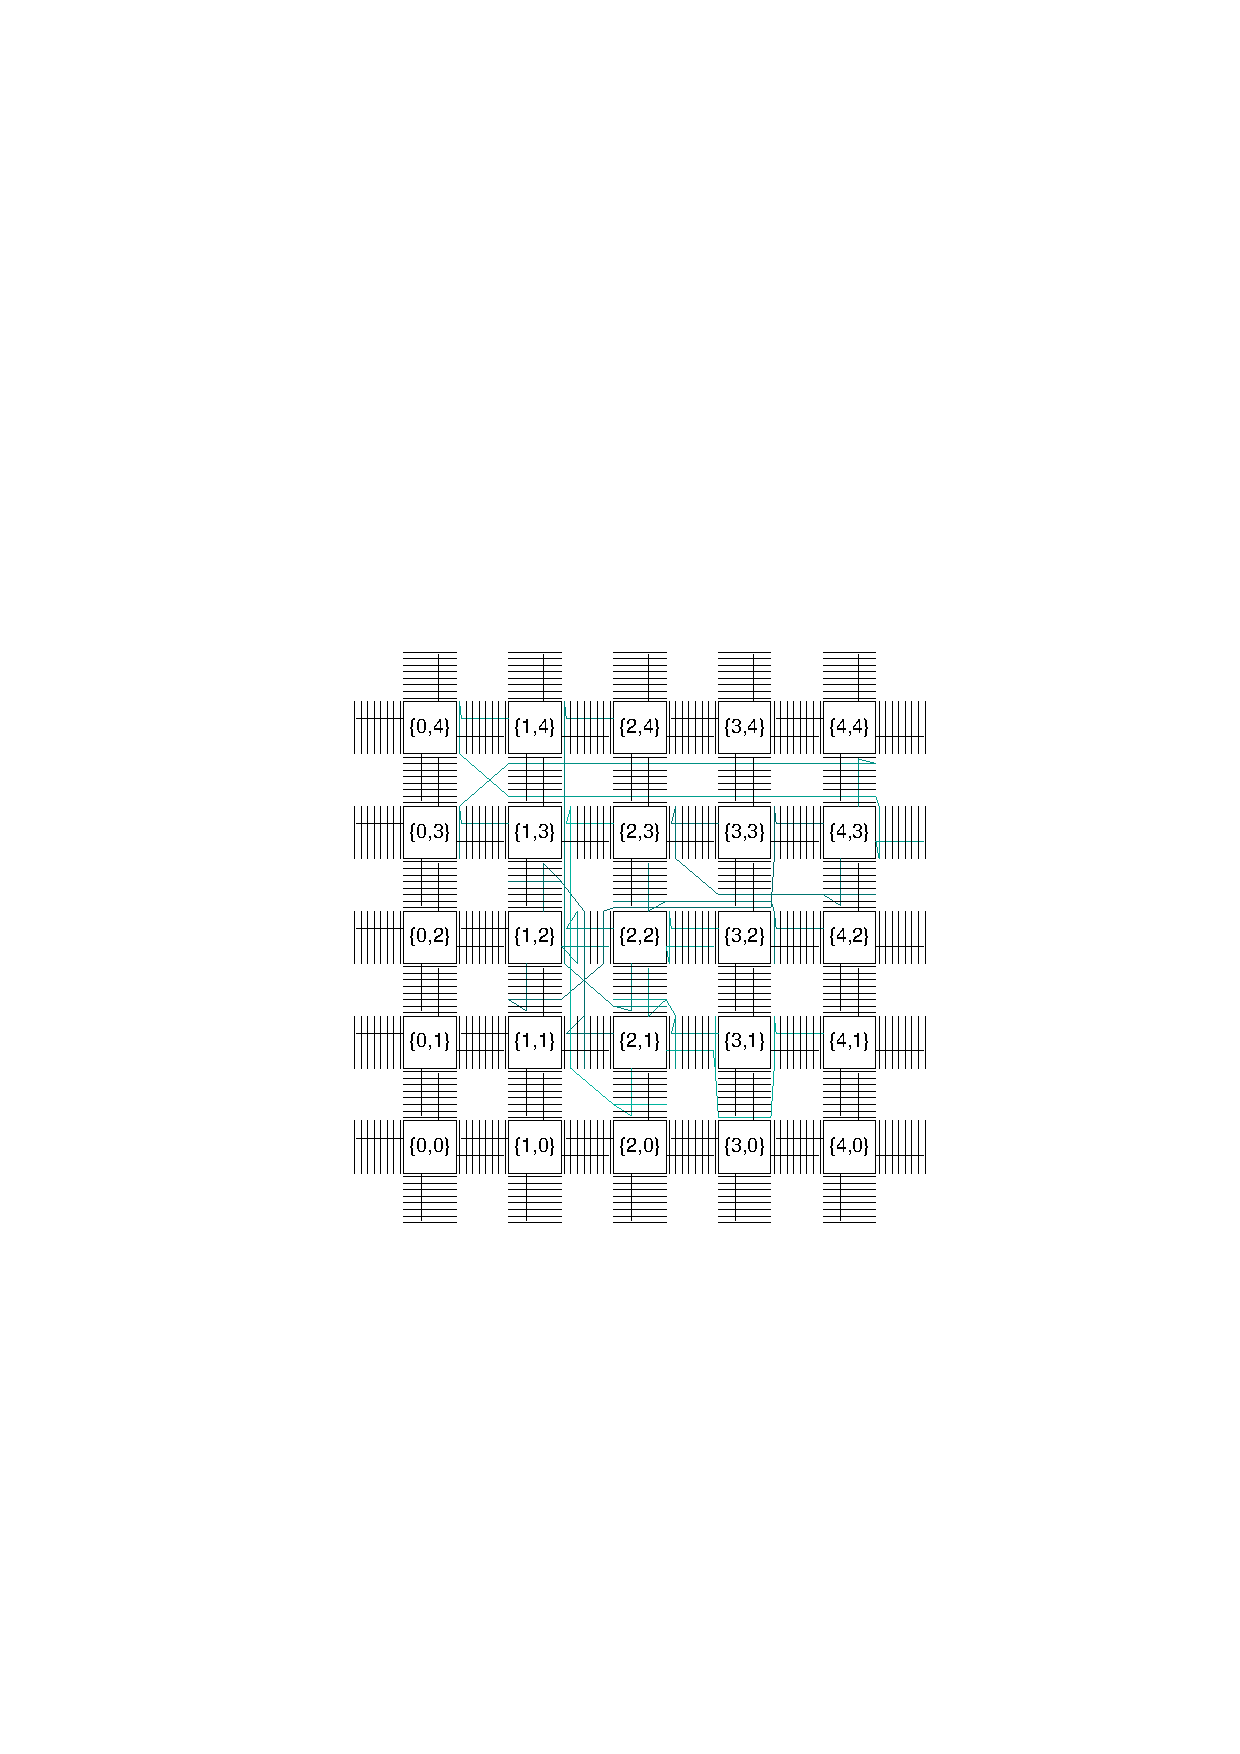
\includegraphics[clip, viewport=170 255 445 529, width=7cm]{assets/wilton-cct1-as-is}
\cprotect\caption{\small\verb|maize-router --data-file ./cct1 --device-type-override wilton-precached --route-as-is --graphics|}
\end{figure}

\subsubsection{Fully Connected}
\begin{figure}[H]
\centering
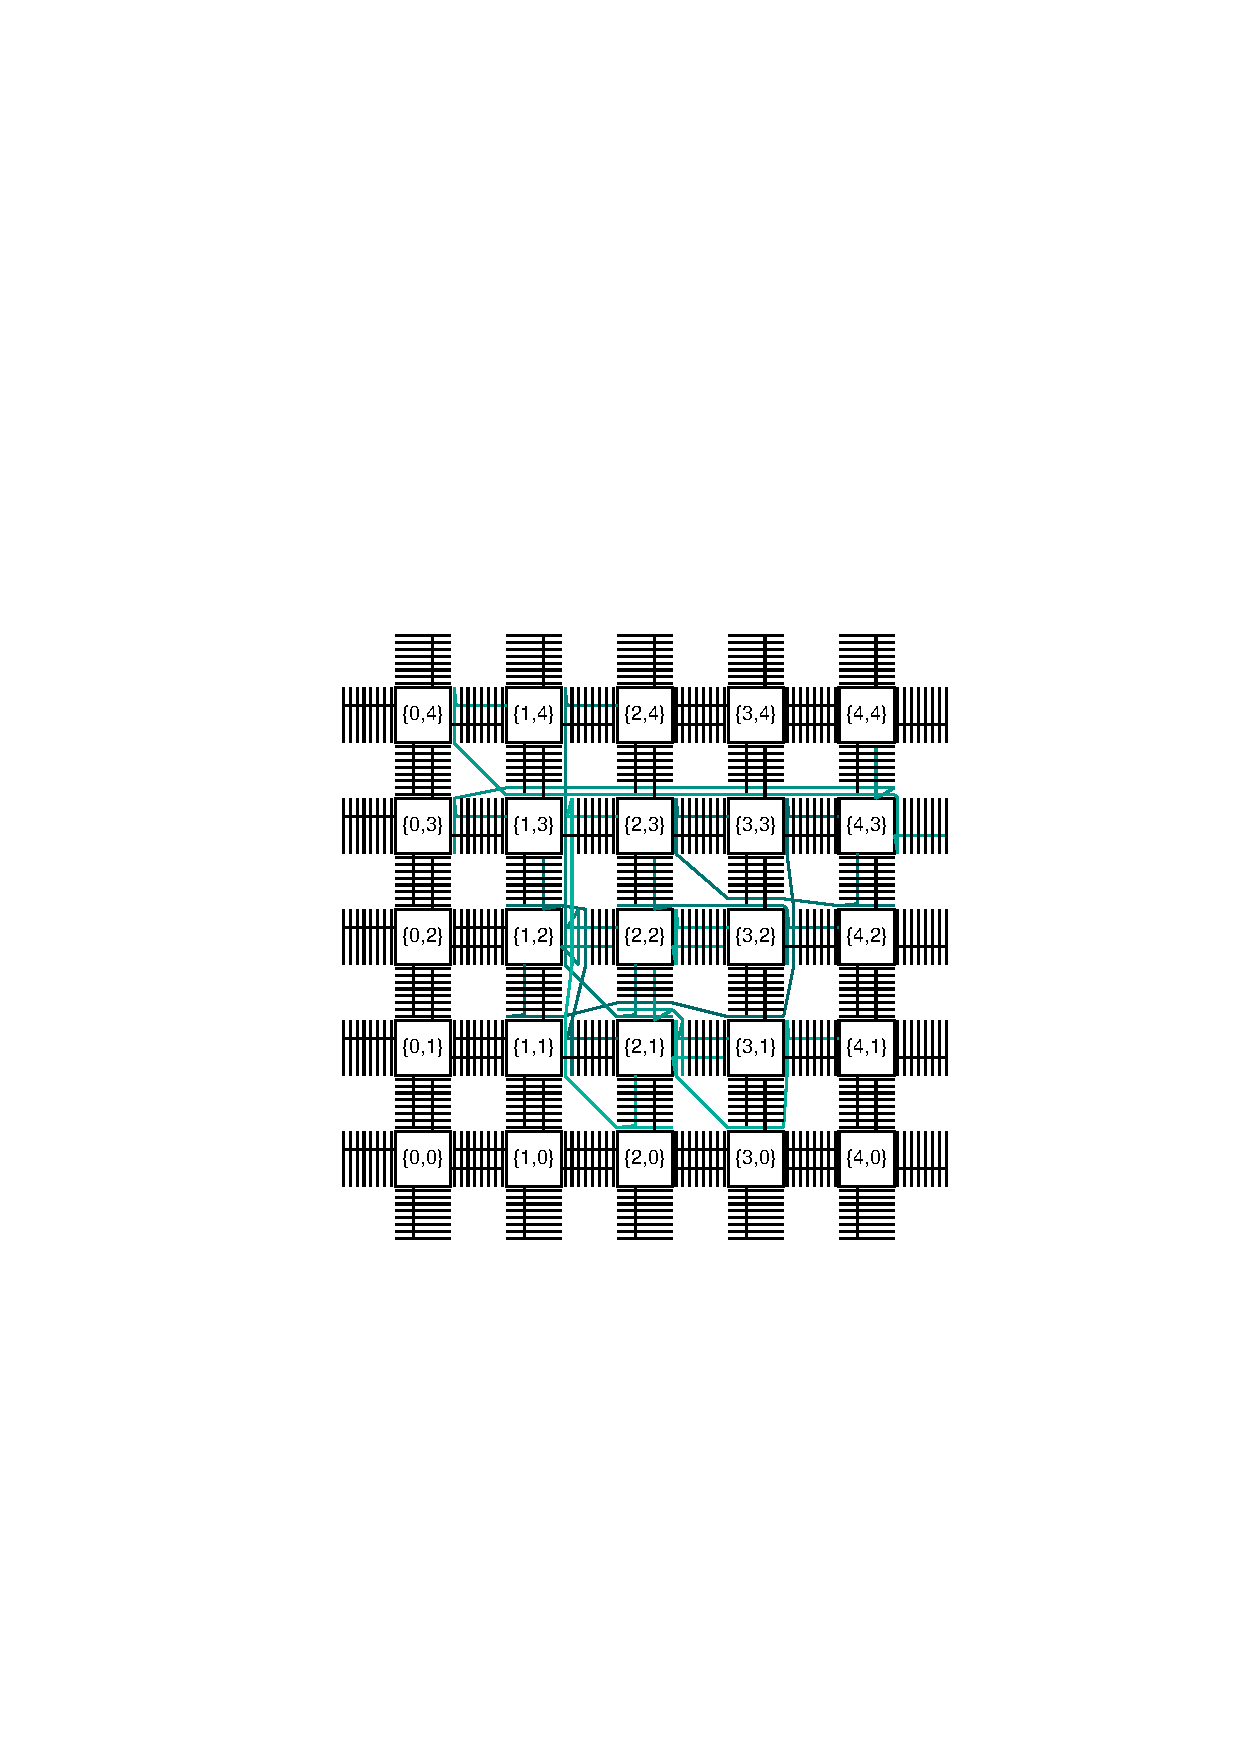
\includegraphics[clip, viewport=164 246 455 538, width=7cm]{assets/fc-cct1-as-is}
\cprotect\caption{\small\verb|maize-router --data-file ./cct1 --device-type-override fc-precached --route-as-is --graphics|}
\end{figure}

\subsection{cct2}
\subsubsection{Wilton}
\begin{figure}[H]
\centering
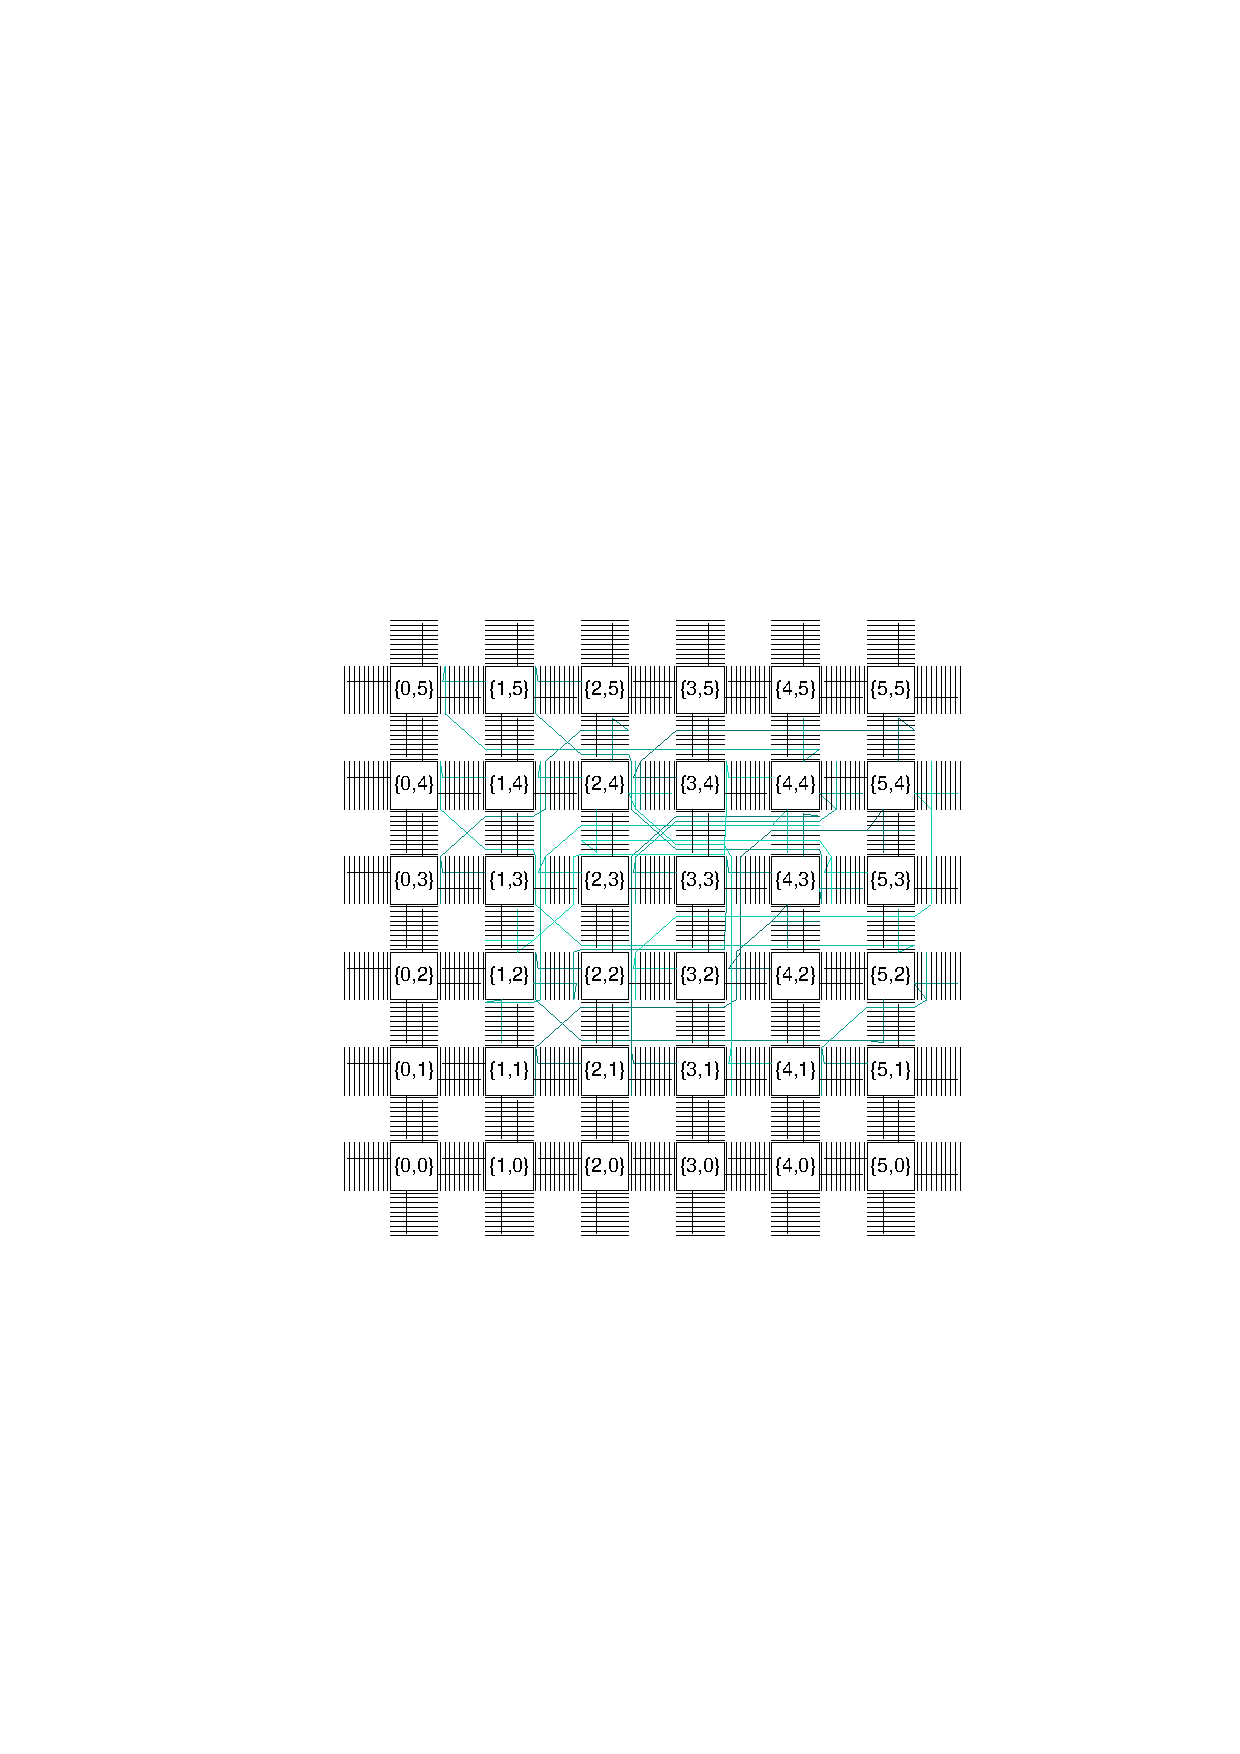
\includegraphics[clip, viewport=165 248 461 544, width=9cm]{assets/wilton-cct2-as-is}
\end{figure}

\subsubsection{Fully Connected}
\begin{figure}[H]
\centering
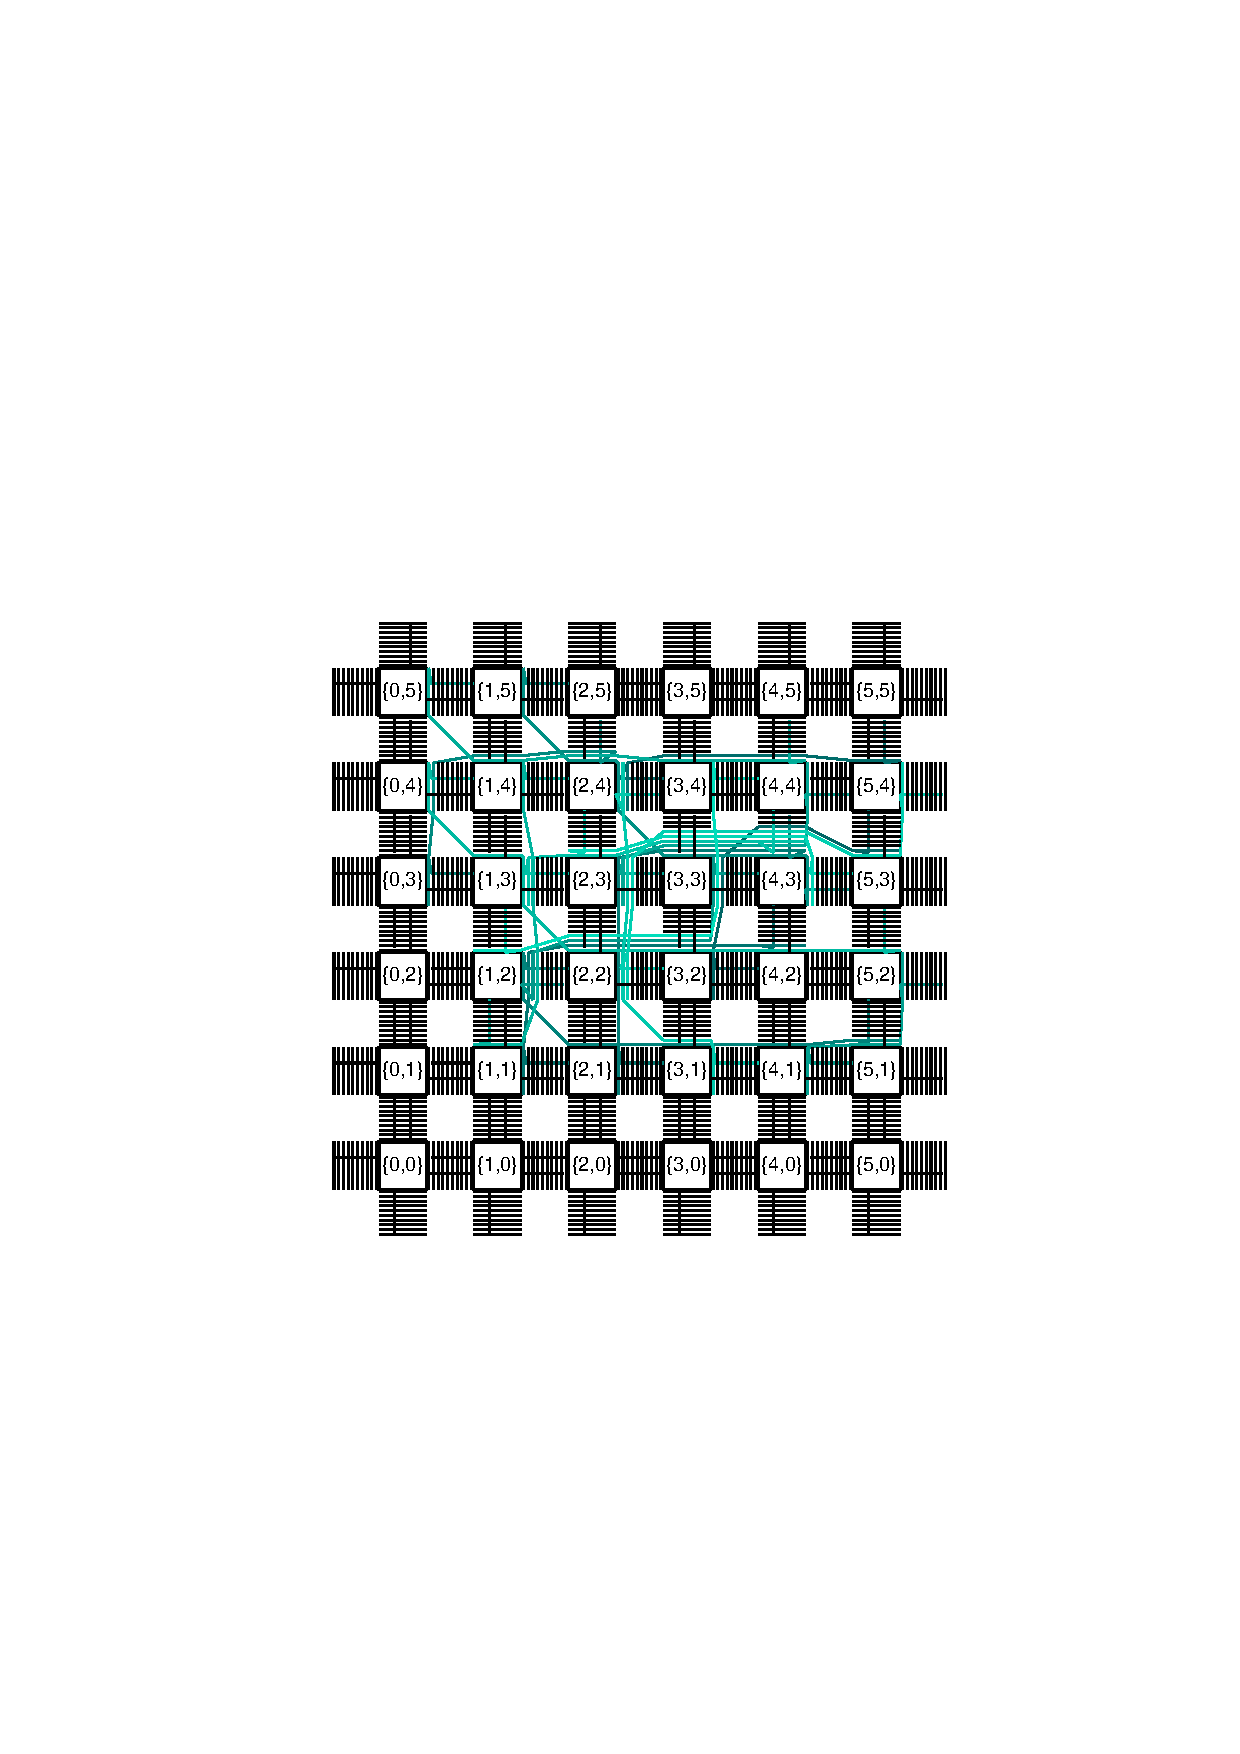
\includegraphics[clip, viewport=159 248 455 544, width=9cm]{assets/fc-cct2-as-is}
\end{figure}

\subsection{cct3}
\subsubsection{Wilton}
\begin{figure}[H]
\centering
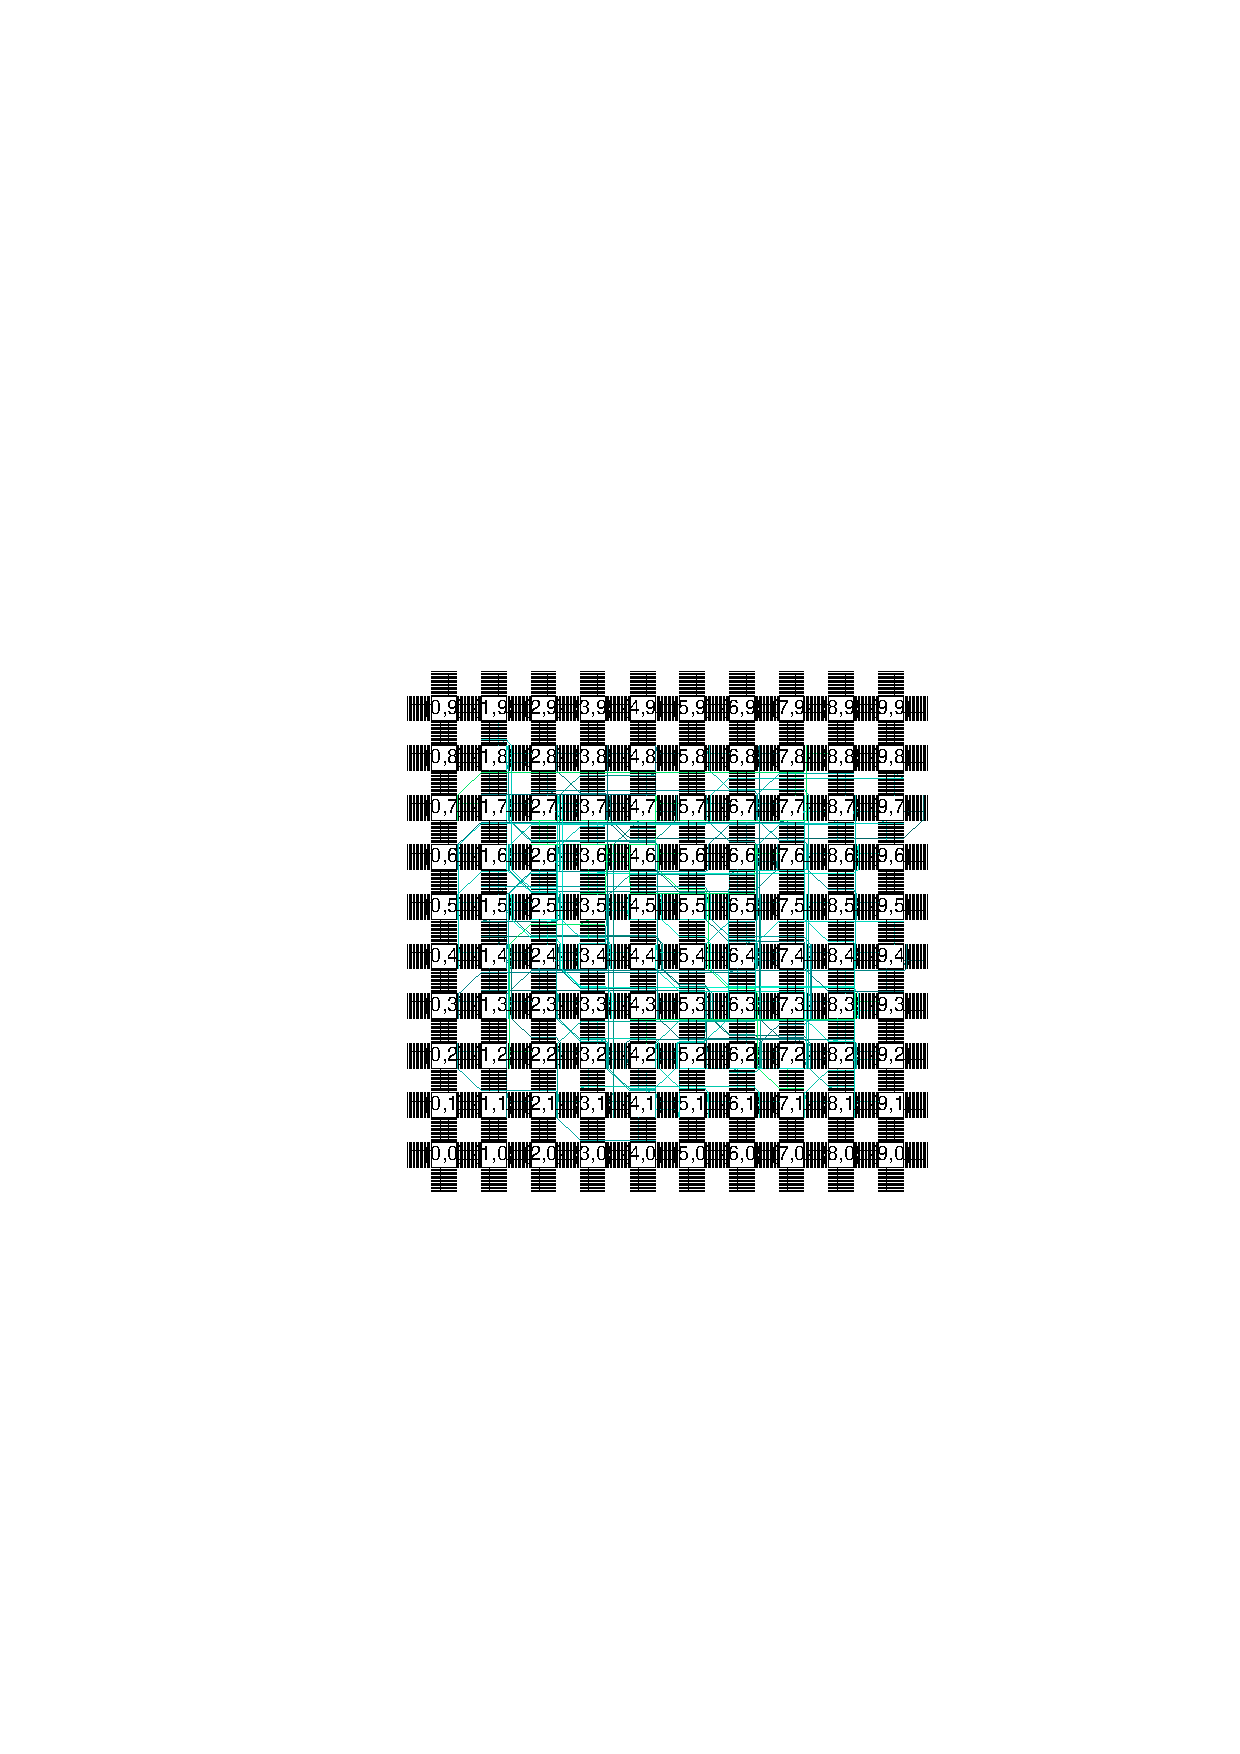
\includegraphics[clip, viewport=195 270 446 520, width=10cm]{assets/wilton-cct3-as-is}
\end{figure}

\subsubsection{Fully Connected}
\begin{figure}[H]
\centering
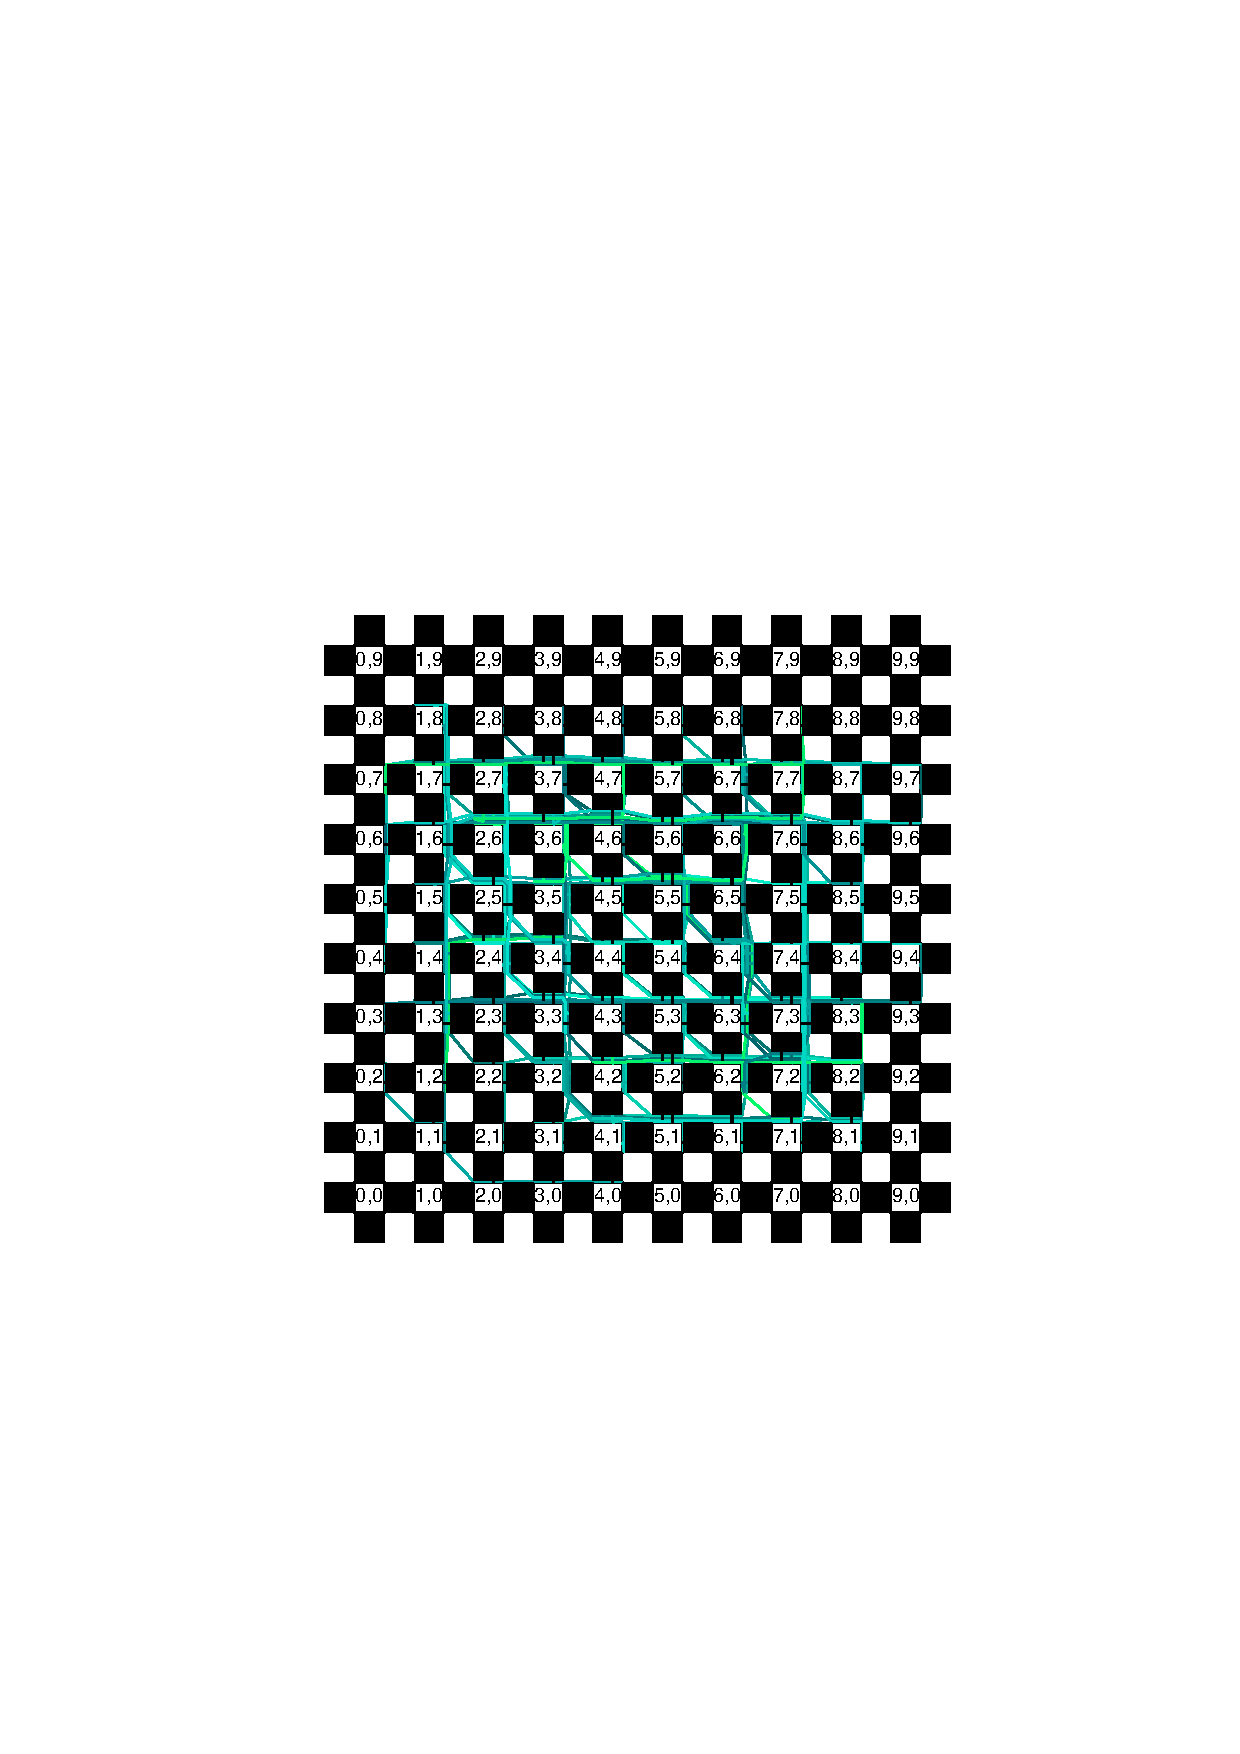
\includegraphics[clip, viewport=155 245 457 547, width=10cm]{assets/fc-cct3-as-is}
\end{figure}

\subsection{cct4}\subsubsection{Wilton}
\begin{figure}[H]
\centering
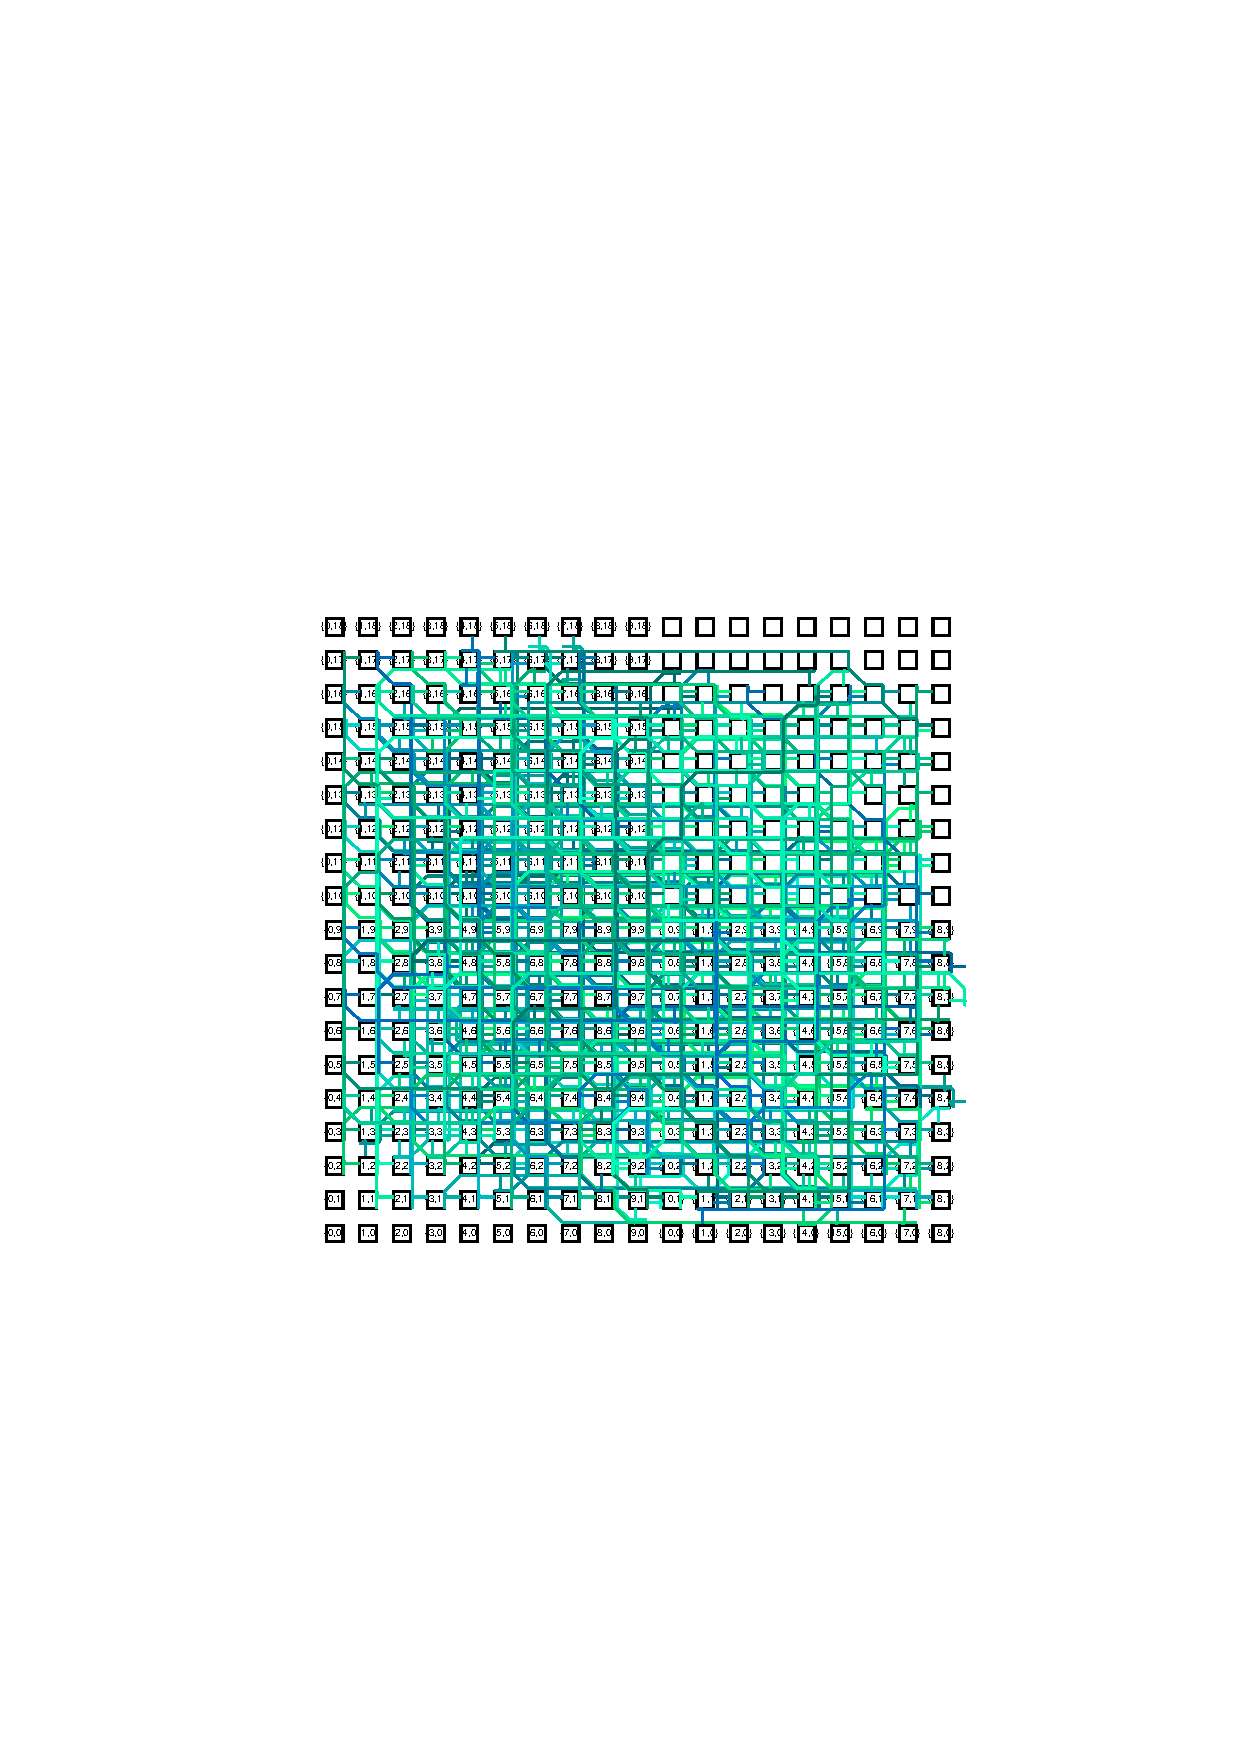
\includegraphics[clip, viewport=154 245 464 546, width=\linewidth]{assets/wilton-cct4-as-is}
\end{figure}

\subsubsection{Fully Connected}
\begin{figure}[H]
\centering
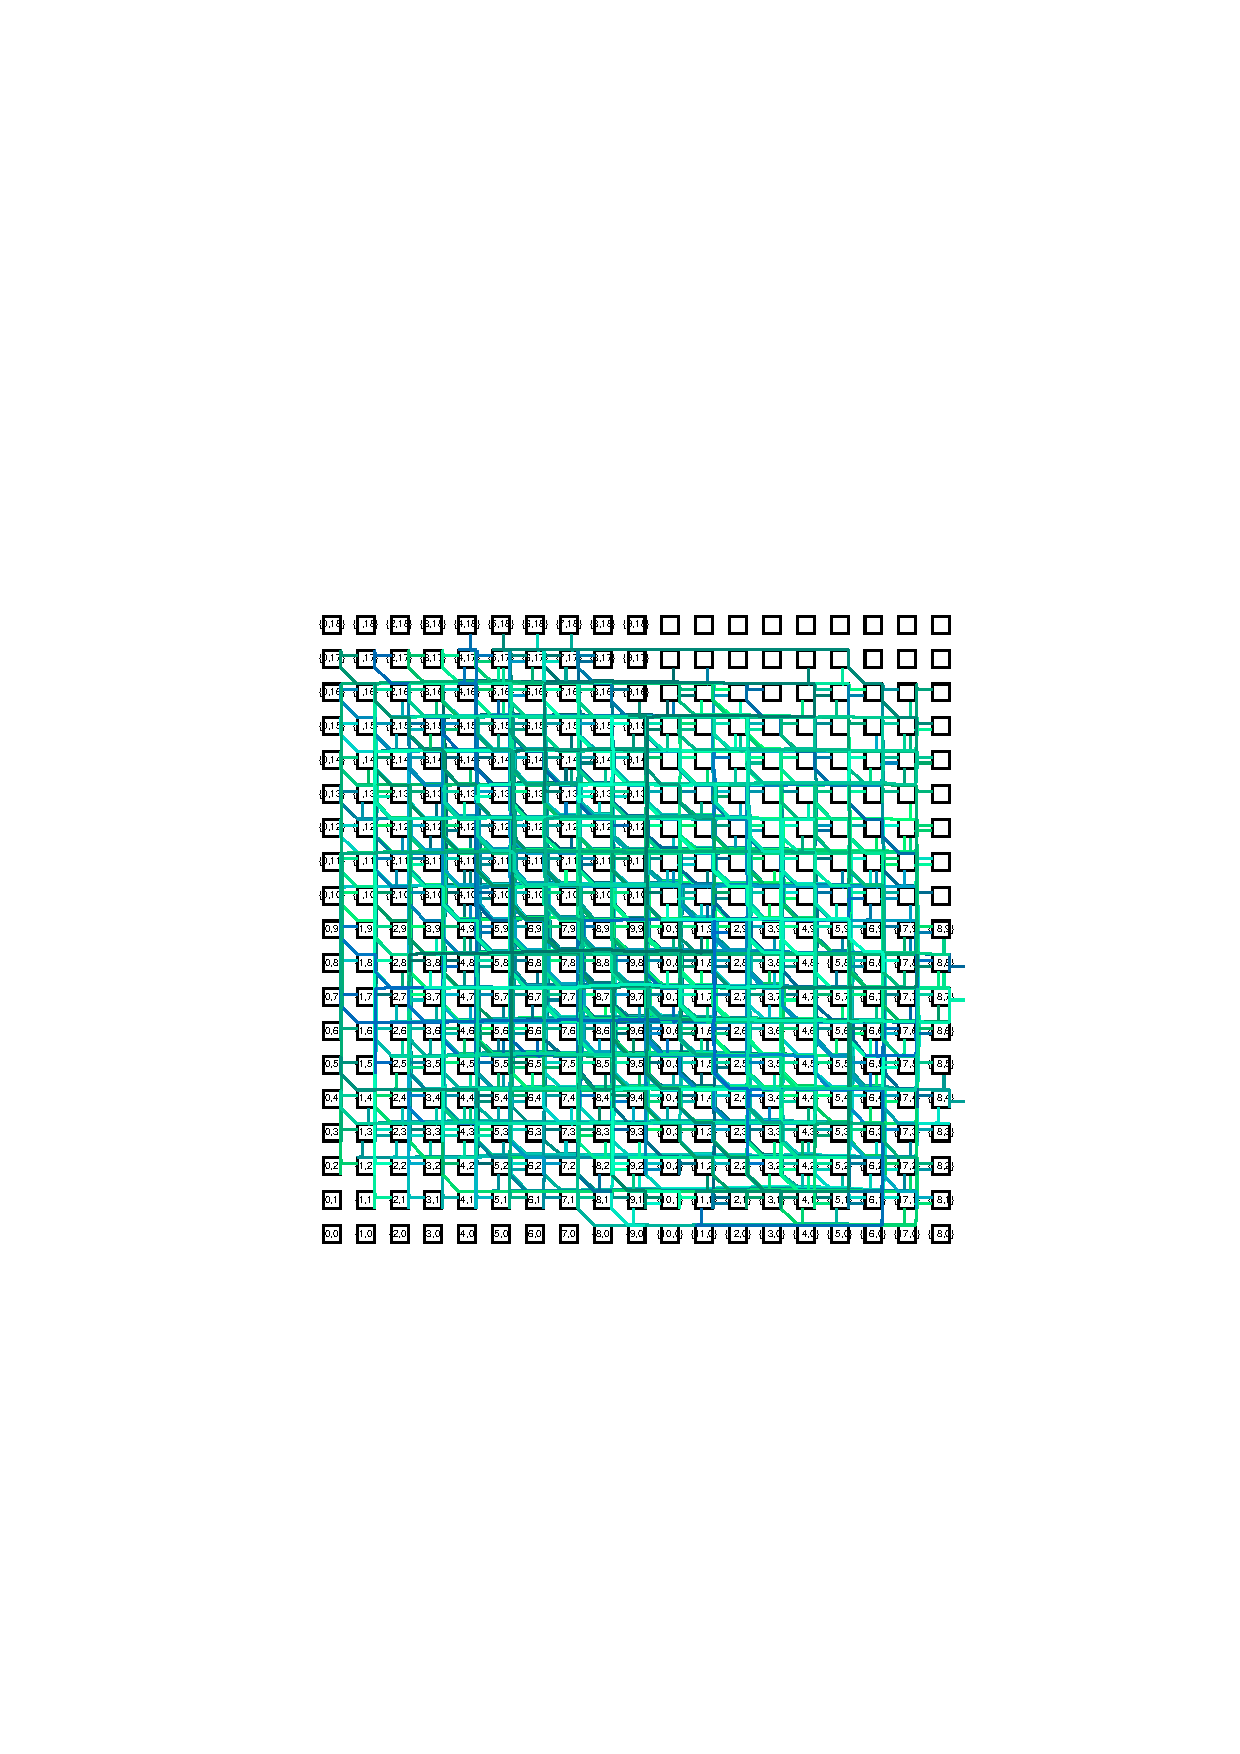
\includegraphics[clip, viewport=153 244 464 547, width=\linewidth]{assets/fc-cct4-as-is}
\end{figure}

\end{document}
